In this section, we will list all the tools and techniques used in this project, the reasons why they are chosen with overall system architecture and the detailed use cases implementations.

\section{System Architecture}
Here, we will continue from the figure \ref{fig:C1} as stated in the Introduction, zooming in to each container and component to see the details of the system architecture.

\paragraph{Level 2: Container diagram}

This is the Container diagram for ComLake Sytem. It shows that the application is made up of 3 containers: a web application Dashboard, a server-side API Application, and a Database. The Dashboard is an ReactJS application that runs in the user's web browser, providing all of the ComLake features. The Dashboard Web Application uses a JSON/HTTP API, which is provided by another Java/Spring MVC application running on the server. The Backend API Application gets user information and other information from the Database (MySQL).

\begin{figure}[H]
    \centering
    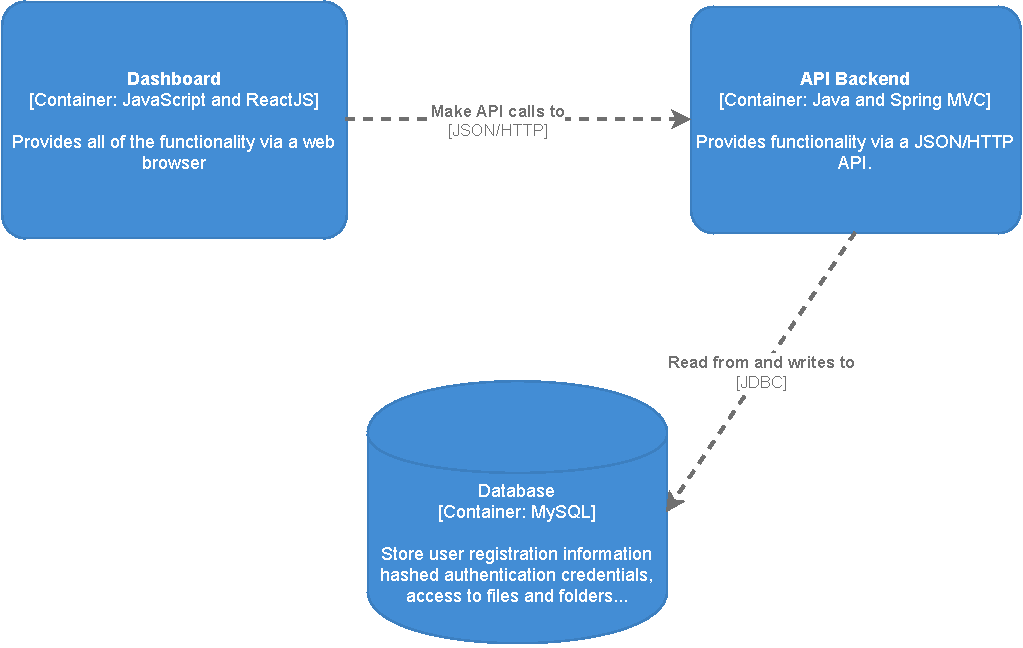
\includegraphics[width=1.0\textwidth]{images/C2.pdf}
    \caption{Container diagram for ComLake System - Backend API and Dashboard}
    \label{fig:C2}
\end{figure}

\paragraph{Level 3: Component diagram}
This is the Component diagram for ComLake system, showing some of the components within the Backend API application. Here, there are six Spring MVC Rest Controllers providing access points for the JSON/HTTP API, with each controller subsequently using other components to access data from the Database.
\begin{figure}[H]
    \centering
    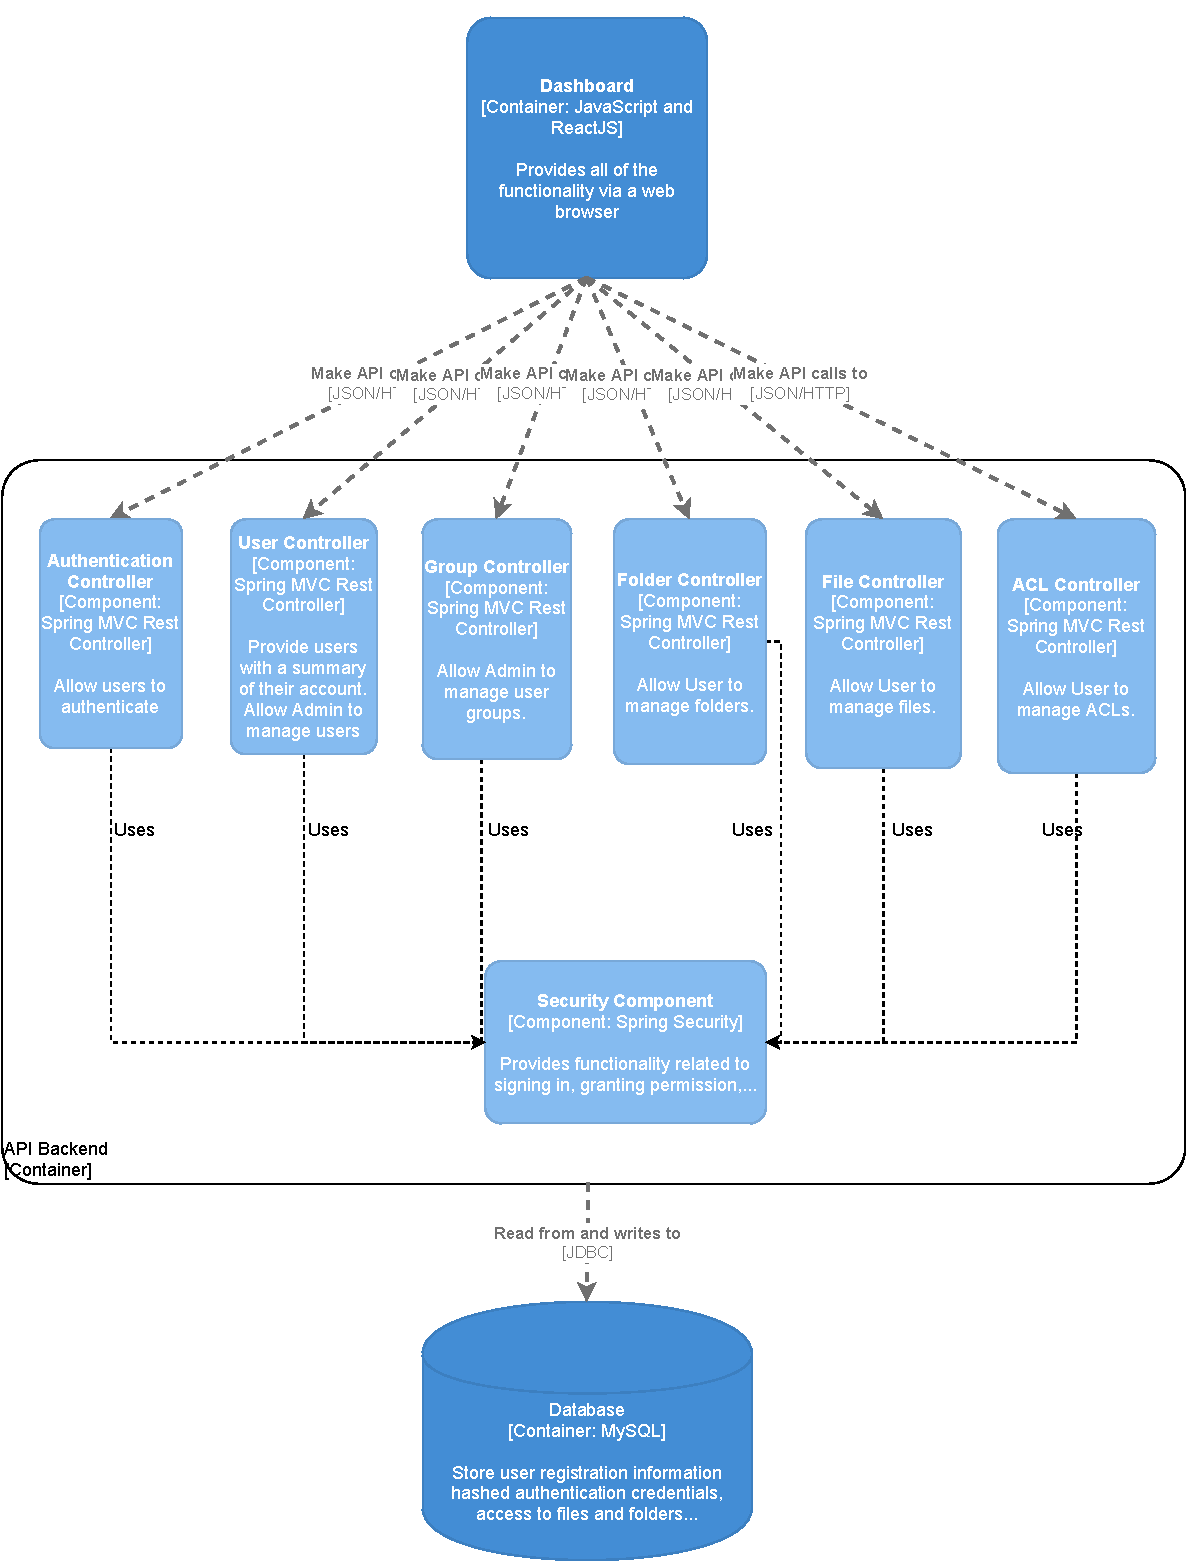
\includegraphics[width=0.9\textwidth]{images/C3.pdf}
    \caption{Component diagram for ComLake Sytem - Backend API}
    \label{fig:C3}
\end{figure}

\paragraph{Level 4: Code}
Finally, this is how the API Backend is implemented as code. This package contains classes for major processing functionality within the system. Control classes exist to support authentication management, user management, user group management, permission management, file and folder management.
\begin{figure}[H]
    \centering
    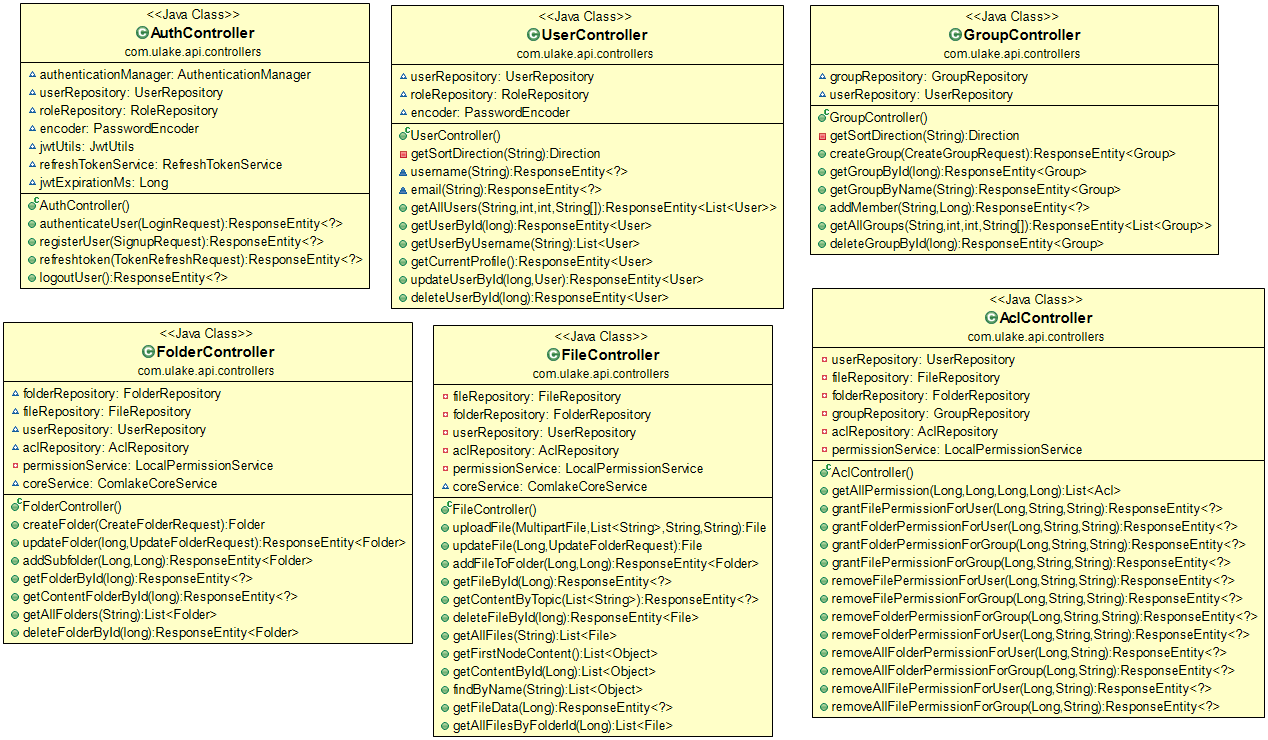
\includegraphics[width=1.0\textwidth]{images/package.png}
    \caption{API Backend Application Package Class diagram}
    \label{fig:C4}
\end{figure}

\section{Database Design}
Every table has the prefix "clake" to distinguish different services of the ComLake service from each other. 

\begin{figure}[H]
    \centering
    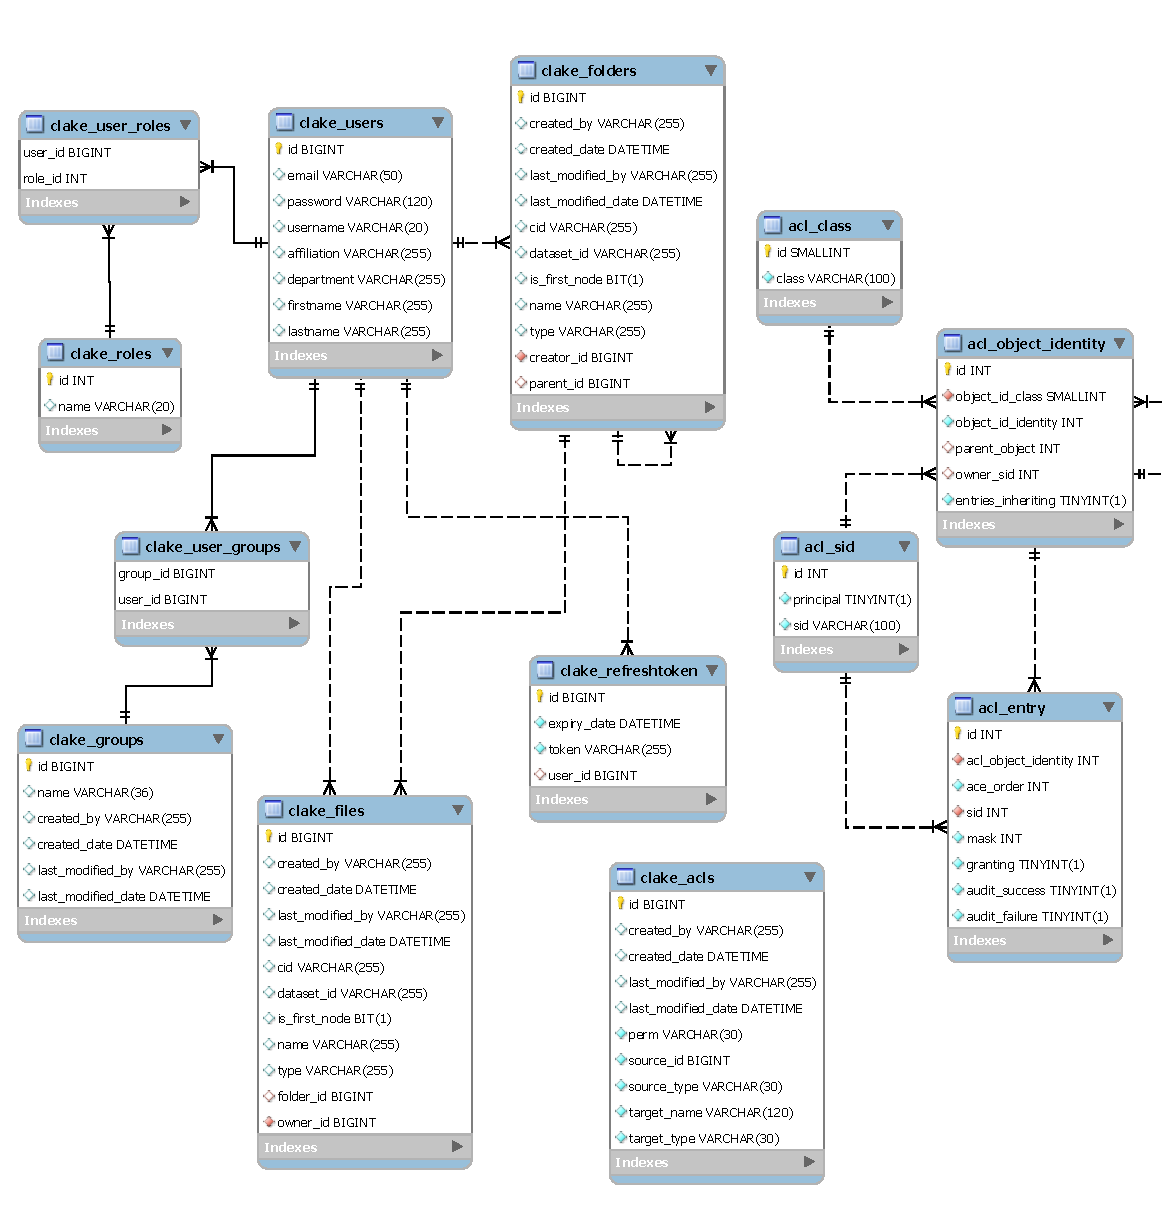
\includegraphics[width=1.0\textwidth]{images/OverallDatabaseDesign.pdf}
    \caption{Overall Database Design}
    \label{fig:DatabaseDesign}
\end{figure}

\begin{table}[H]
  \centering
  \caption{Database User Design}
  \label{tbl:dbUser}
  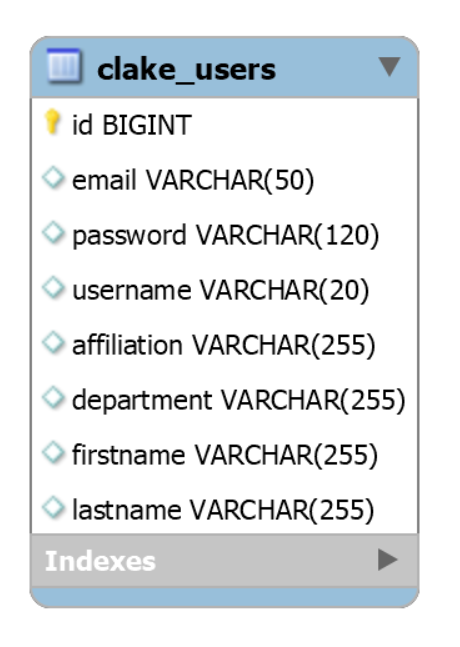
\includegraphics[width=0.3\textwidth]{images/DatabaseUserDesign.PNG}
\end{table}
\begin{itemize}
    \item "clake\_users" is the table that contains the information of accounts. This table has sensitive data of users such as "password". 
    \item The 'password' field in this table is saved in an encrypted form not easily used by attackers. 
    \item After the user register, the system saves the user information and assign a unique "id" to the user, and this "id" is the Primary key of the table. 
\end{itemize}

\begin{table}[H]
  \centering
  \caption{Database Role Design}
  \label{tbl:dbRole}
  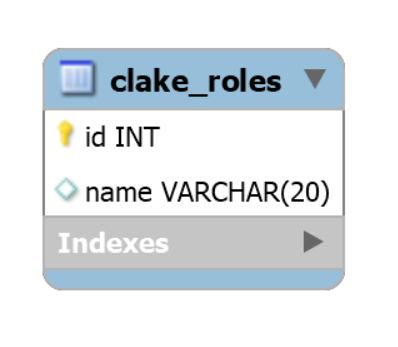
\includegraphics[width=0.3\textwidth]{images/DatabaseRoleDesign.PNG}
\end{table}
\begin{itemize}
    \item "clake\_roles" is the table that contains the information of roles, for example role name. 
    \item In this system, we only have 2 role. Role Admin and role (Regular) User.
    \item This table has "id" as Primary Key. Each role has an unique "id". 
\end{itemize}

\begin{table}[H]
  \centering
  \caption{Database User Role Design}
  \label{tbl:dbUserRole}
  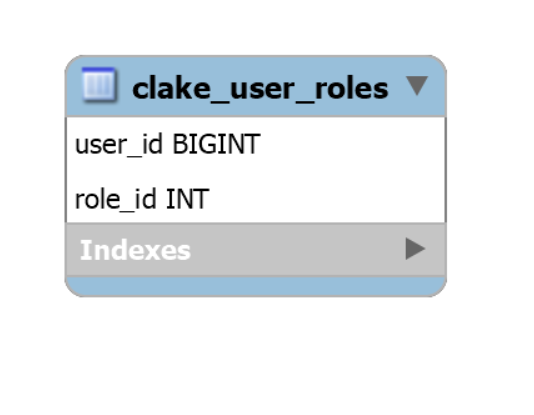
\includegraphics[width=0.3\textwidth]{images/DatabaseUserRoleDesign.PNG}
\end{table}
\begin{itemize}
    \item "clake\_user\_roles" is a table containing user and their associated role.
    \item This table connects with the "clake\_users" table and "clake\_roles" table with the Foreign Key: 'user\_id' and 'role\_id'. This is "many to many" relationship: Each "User" could have many roles. Each "Role" could have many users.  
\end{itemize}

\begin{table}[H]
  \centering
  \caption{Database Group Design}
  \label{tbl:dbGroup}
  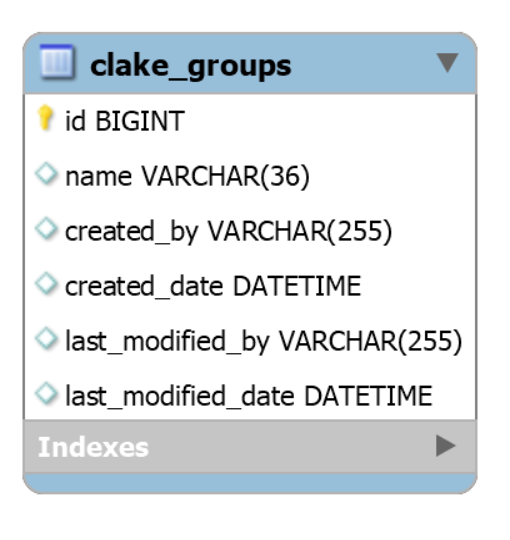
\includegraphics[width=0.3\textwidth]{images/DatabaseUserGroupDesign.PNG}
\end{table}
\begin{itemize}
    \item "clake\_groups" is the table that contains the information of groups, for example group name. 
    \item This table has "id" as Primary Key. Each group has an unique "id". 
    \item Group name must be unique from each other.
    \item This table is audit-able, by the field 'created\_by', 'created\_date', 'last\_modified\_by' and 'last\_modified\_date'. It will monitoring and recording of selected user database actions.
\end{itemize}

\begin{table}[H]
  \centering
  \caption{Database User Group Design}
  \label{tbl:dbUserGroup}
  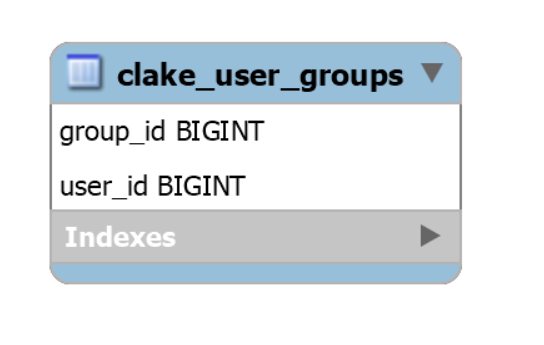
\includegraphics[width=0.3\textwidth]{images/DatabaseUserAGroupDesign.PNG}
\end{table}
\begin{itemize}
    \item "clake\_user\_groups" is a table containing user and their associated group.
    \item This table connects with the "clake\_users" table and "clake\_groups" table with the Foreign Key: 'user\_id' and 'group\_id'. This is "many to many" relationship: Each "User" could have many groups. Each "Group" could have many users.  
\end{itemize}

\begin{table}[H]
  \centering
  \caption{Database Refresh Token Design}
  \label{tbl:dbRefreshToken}
  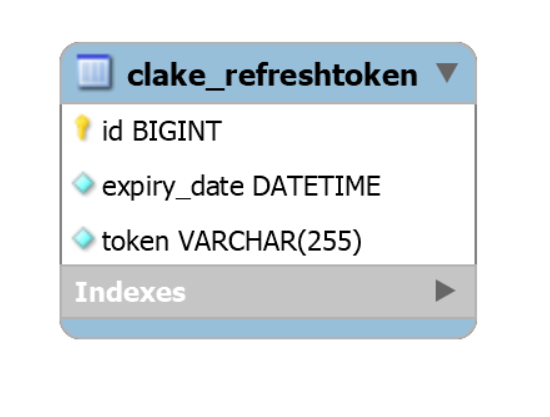
\includegraphics[width=0.3\textwidth]{images/DatabaseRefreshTokenDesign.PNG}
\end{table}
\begin{itemize}
    \item "clake\_refreshtoken" is the table that contains the refresh token information of an user.
    \item This will keep user logged in longer time with silent authentication because it has longer expiry date than the access token. 
    \item This table has "id" as Primary Key.
    \item This has one-to-one relationship with "User".
\end{itemize}

\begin{table}[H]
  \centering
  \caption{Database Folder Design}
  \label{tbl:dbFolder}
  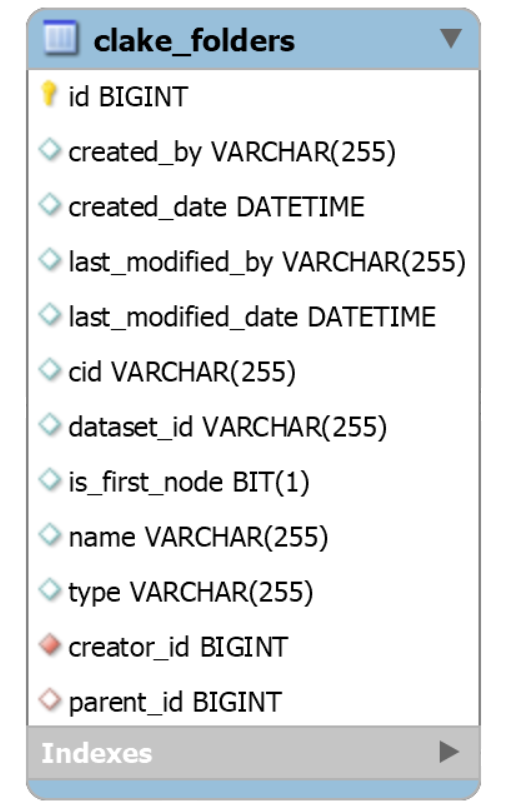
\includegraphics[width=0.3\textwidth]{images/DatabaseFolderDesign.PNG}
\end{table}
\begin{itemize}
    \item "clake\_folders" is the table that contains the information of folders.
    \item This table has "id" as Primary Key. Each folder has an unique "id". 
    \item This table connects with the "clake\_users" table with the Foreign Key 'creator\_id'. This is "many to one" relationship: Many "Folder" belongs to a "User". 
    \item The column 'parent\_id' is a foreign key that refers to the primary key column 'id' of the table itself. This is parent-child relationship, it needed to represent nested, hierarchical structures: A "Folder" can have one or many children folders below it. And vice-versa, a "Folder" can have one or many parent folders above it. There is no limit for the nested level.
    \item Noted that this table doesn't include 'source' and 'topics' fields because that metadata is stored in the ComLake Core. We use 'cid' and 'dataset\_id' as identifier to connect to the Core. 
    \item This table is audit-able, by the field 'created\_by', 'created\_date', 'last\_modified\_by' and 'last\_modified\_date'. It will monitoring and recording of selected user database actions.
\end{itemize}
\begin{table}[H]
  \centering
  \caption{Database File Design}
  \label{tbl:dbFile}
  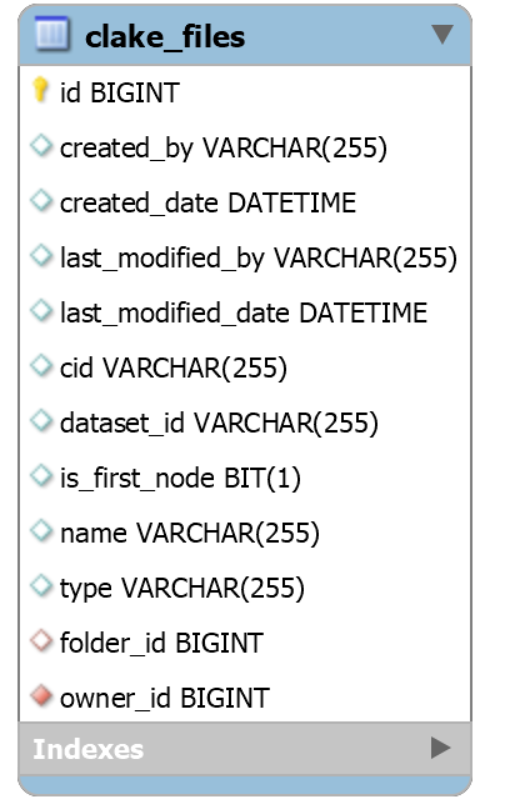
\includegraphics[width=0.3\textwidth]{images/DatabaseFileDesign.PNG}
\end{table}
\begin{itemize}
    \item "clake\_files" is the table that contains the information of files.
    \item This table has "id" as Primary Key. Each file has an unique "id". 
    \item This table connects with the "clake\_users" table with the Foreign Key 'owner\_id'. This is "many to one" relationship: Many "File" belongs to a "User".
    \item This table connects with the "clake\_folders" table with the Foreign Key 'folder\_id'. This is "many to one" relationship: Many "File" could be in a "Folder". 
    \item Noted that this table doesn't include 'source' and 'topics' fields because that metadata is stored in the ComLake Core. We use 'cid' and 'dataset\_id' as identifier to connect to the Core. 
    \item This table is audit-able, by the field 'created\_by', 'created\_date', 'last\_modified\_by' and 'last\_modified\_date'. It will monitoring and recording of selected user database actions.
\end{itemize}

\begin{table}[H]
  \centering
  \caption{Database ACL Class Design}
  \label{tbl:dbACL}
  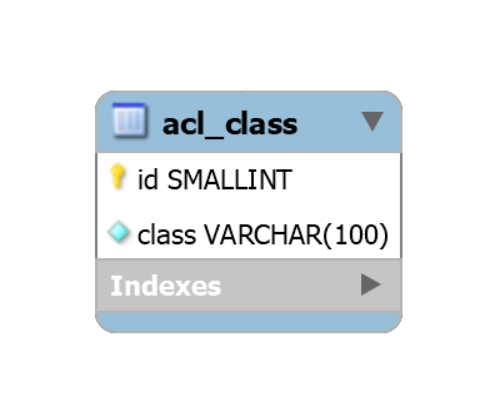
\includegraphics[width=0.3\textwidth]{images/DatabaseAclClassDesign.PNG}
\end{table}
\begin{itemize}
    \item "acl\_class" is the table that stores the class name of the domain object. 
    \item This table has "id" as Primary Key. Each file has an unique "id".
    \item In this system, we only have two classes that need to be secured: "File" and "Folder". So it will store two values: "com.ulake.api.models.File" and "com.ulake.api.models.Folder". 
\end{itemize}

\begin{table}[H]
  \centering
  \caption{Database ACL Sid Design}
  \label{tbl:dbACL}
  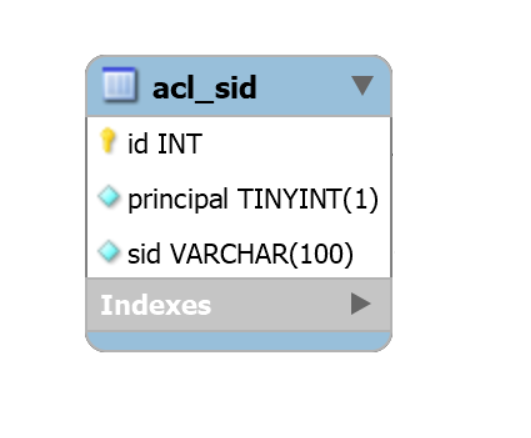
\includegraphics[width=0.3\textwidth]{images/DatabaseAclSidDesign.PNG}
\end{table}
\begin{itemize}
    \item "acl\_sid" is the table that allows us to universally identify any users, roles or groups in the system. 
    \item This table has "id" as Primary Key. Each file has an unique "id".
    \item The field 'sid' could be username of the user or role name like "ROLE\_ADMIN" or group name. SID stands for "Security Identity".
    \item The field 'principal' could be 0 or 1. It is a Boolean value indicate if the corresponding 'sid' is a principal (user) or an authority (role or group). 
\end{itemize}

\begin{table}[H]
  \centering
  \caption{Database ACL Object Identity Design}
  \label{tbl:dbACL}
  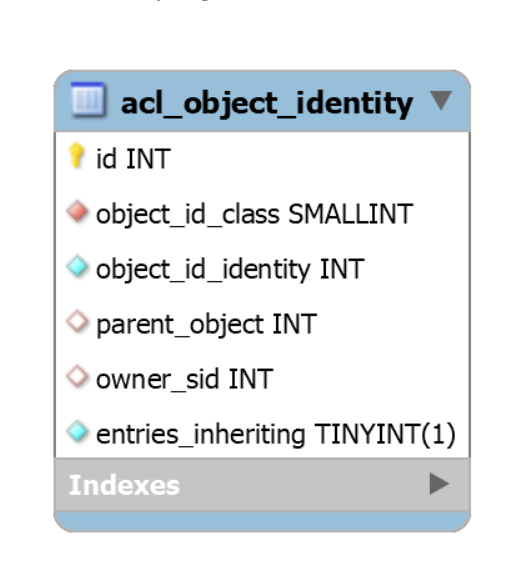
\includegraphics[width=0.3\textwidth]{images/DatabaseAclOIDesign.PNG}
\end{table}
\begin{itemize}
    \item "acl\_object\_identity" is the table that stores the information for each unique domain object (File or Folder). 
    \item This table has "id" as Primary Key. Each file has an unique "id".
    \item The field 'object\_id\_class' indicate if it is File or Folder.
    \item The field 'owner\_sid' links to "acl\_sid" table. It is the Id of the owner. 
\end{itemize}

\begin{table}[H]
  \centering
  \caption{Database ACL Entry}
  \label{tbl:dbACL}
  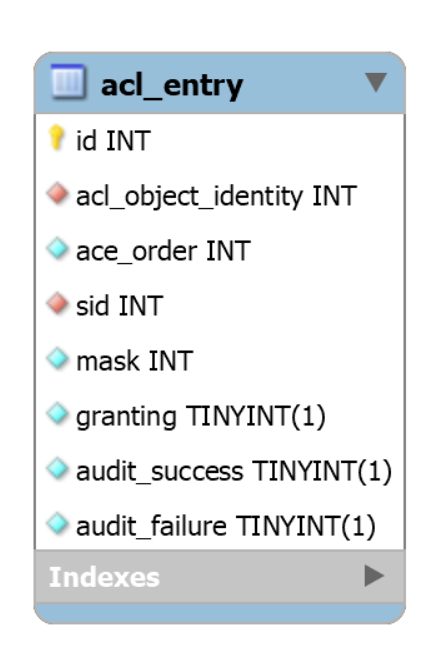
\includegraphics[width=0.3\textwidth]{images/DatabaseAclEntryDesign.PNG}
\end{table}
\begin{itemize}
    \item "acl\_entry" is the table that stores individual permission assigns to each SID on an Object Identity.
    \item This table has "id" as Primary Key. Each file has an unique "id".
    \item The field 'acl\_object\_identity' specify the object identity, links to "acl\_object\_identity" table. 
    \item The field 'ace\_order' is the order of current entry in the ACL entries list of corresponding Object Identity.
    \item The field 'sid' is the target SID which the permission is granted to or denied from, links to "acl\_sid" table.
\end{itemize}

\begin{table}[H]
  \centering
  \caption{Database ACL Design}
  \label{tbl:dbACL}
  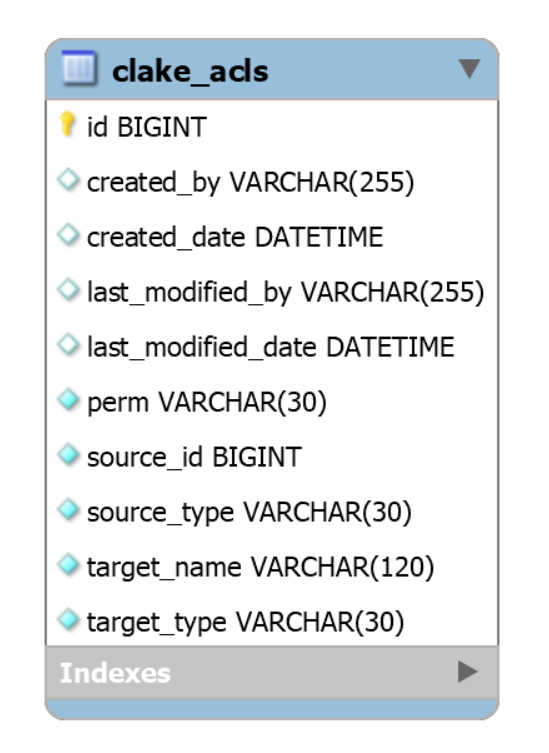
\includegraphics[width=0.3\textwidth]{images/DatabaseAclDesign.PNG}
\end{table}
\begin{itemize}
    \item "clake\_acls" is the table that mimics the table "acl\_entry" for easier interface.
    \item This table has "id" as Primary Key. Each file has an unique "id".
    \item The field 'source\_type' could be "File" or "Folder".
    \item The field 'target\_type' could be "User" or "Group". 
    \item The field 'perm' could be "Read" or "Write". 
    \item This table is audit-able, by the field 'created\_by', 'created\_date', 'last\_modified\_by' and 'last\_modified\_date'. It will monitoring and recording of selected user database actions.
\end{itemize}
\section{Use Cases Implementation}
\subsection{Login}
This use case describes how a user logs into the system. This user can be a Admin or a (Regular) User. When a user wants to login, the system requests the actor to enter username and password (Figure \ref{fig:login} in Appendices). Once the user enters the username and password, the system will check if the information is valid and logs the user in. Otherwise, the system displays and error message and asks the user to re-enter the information. 
\begin{figure}[H]
    \centering
    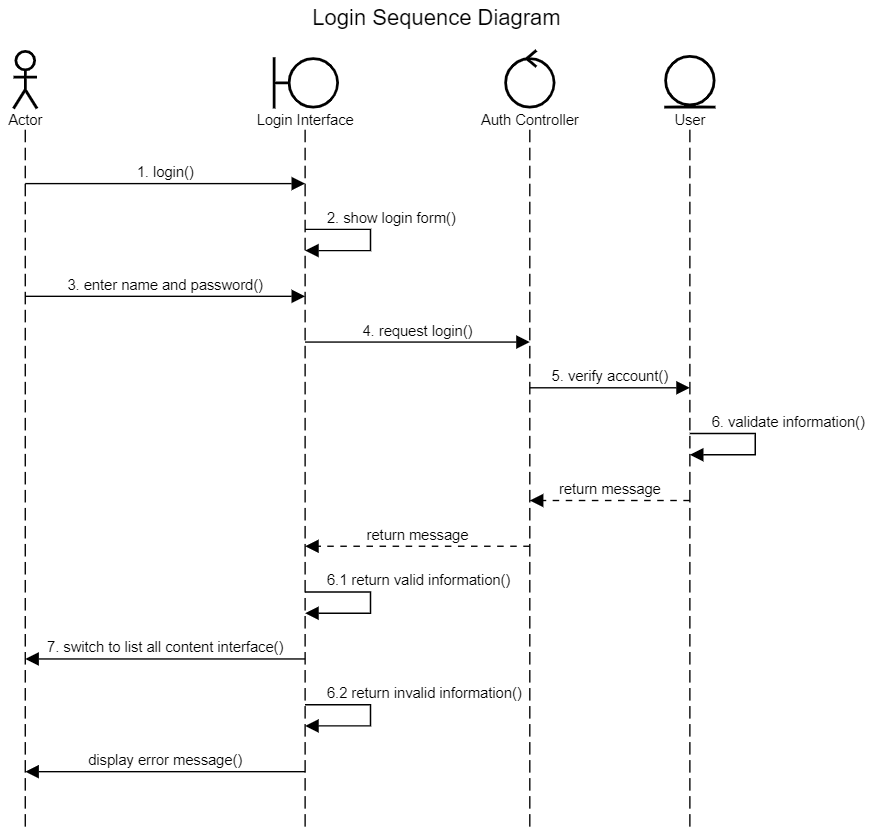
\includegraphics[width=1.0\textwidth]{images/LoginSequence.png}
    \caption{Login Sequence diagram}
    \label{fig:LoginSeq}
\end{figure}

\subsection{Register}
This use case describes how a user registers to the system. When a user wants to register into the system, the system will display a register interface and requests that the user enter first name, last name, email, username, and password (Figure \ref{fig:register} in Appendices). After the user enters the required information, the system checks if the entered email and username are unique from the table "comlake\_users" in Database. If unique, the system encrypts the password, saves the user information, assigns a unique id to the user, and redirects to the login interface. Otherwise, the system displays an error message and asks the user to re-enter the information.

\begin{figure}[H]
    \centering
    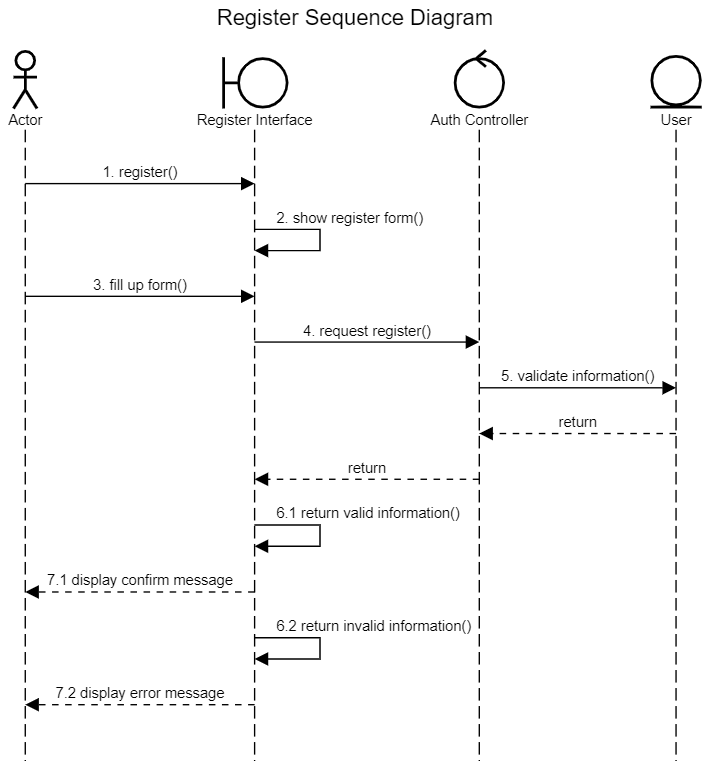
\includegraphics[width=1.0\textwidth]{images/RegisterSequence.png}
    \caption{Register Sequence diagram}
    \label{fig:RegisterSeq}
\end{figure}

\subsection{Manage Users}
This Use Case describes how an Admin can manage users.

\subsubsection{Manage Users - Basic flow}
When the Admin logged into the system, there will be a User tab if the Admin wishes to manage users. The system lists all of the users (Figure \ref{fig:adminAllUsers} in Appendices). The Admin can filter users with desired criteria, and the system will respond to a list of users according to the criteria. The Admin could choose to perform an action (create, edit, delete). If the Admin chooses to create a user, there will be a create user form (Figure \ref{fig:adminCreateUser} in Appendices). After the Admin enters the required information, the system checks if the entered email and username are unique from the table "comlake\_users" in Database. If unique, the system encrypts the password, saves the user information, assigns a unique id to the user, and redirects to the login interface. Otherwise, the system displays an error message and asks the Admin to re-enter the information. 
\begin{figure}[H]
    \centering
    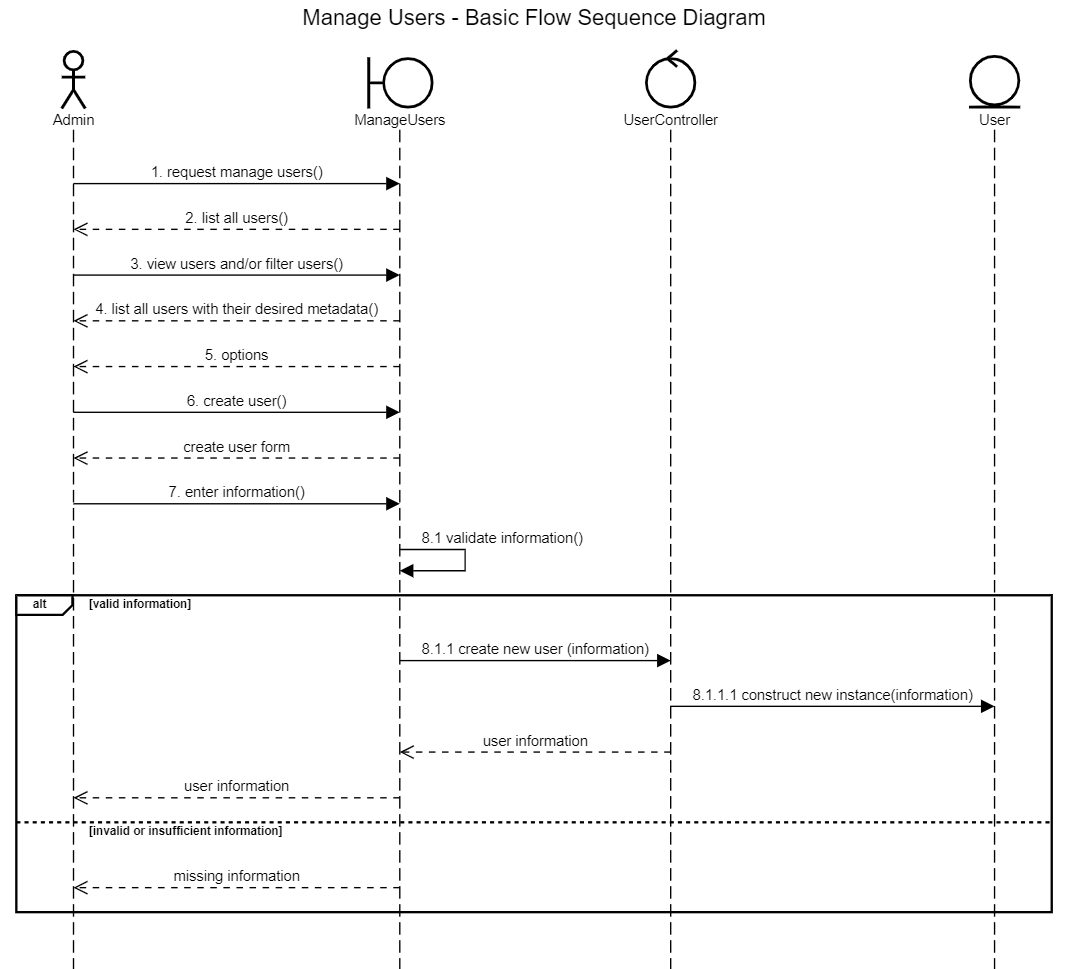
\includegraphics[width=1.0\textwidth]{images/Manage Users - Basic Flow Sequence Diagram.png}
    \caption{Manage Users - Basic Flow Sequence diagram}
    \label{fig:SeqUsersBasic}
\end{figure}

\subsubsection{Update User - Sub flow}
If the Admin wishes to edit a user by select the target user, the system will display an update user form (Figure \ref{fig:adminEditDeleteUser} in Appendices). After the Admin enters the updated information, the system will check if the user exists or not. If the user exists, the system will save the updated information of the user. If not, the system displays an error message. 

\begin{figure}[H]
    \centering
    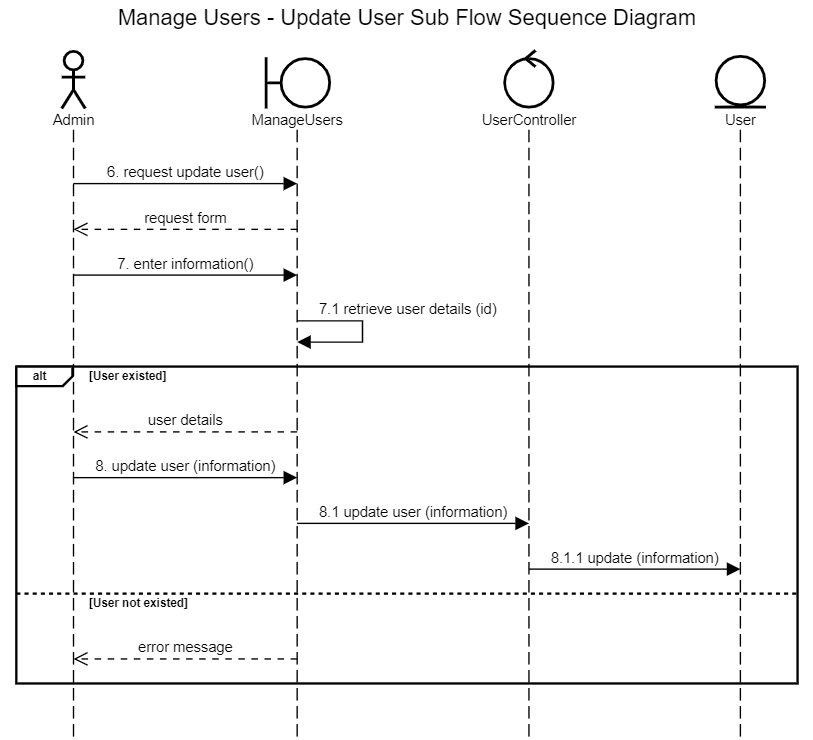
\includegraphics[width=1.0\textwidth]{images/Manage Users - Update User Sub Flow Sequence Diagram.png}
    \caption{Manage Users - Update User Sub Flow Sequence diagram}
    \label{fig:SeqUsersUpdate}
\end{figure}

\subsubsection{Delete User - Sub flow}
If the Admin wished to delete a user by selecting the target user, the system would display the full details of the user. When Admin clicks on the "Delete" button, the system will checks if the user exists or not. If the user exists, the system will remove the user. If not, the system displays an error message.
\begin{figure}[H]
    \centering
    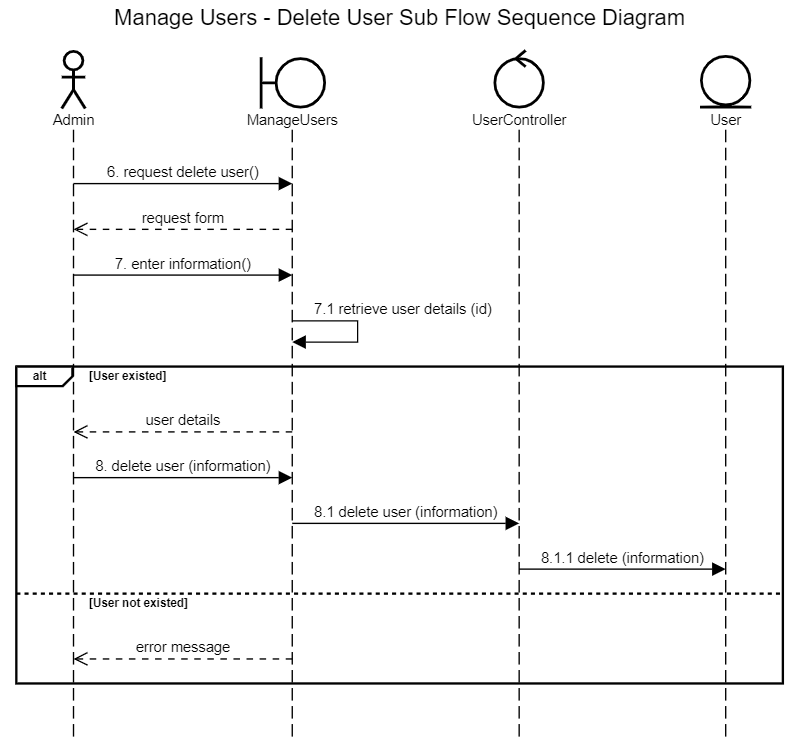
\includegraphics[width=1.0\textwidth]{images/Manage Users - Delete User Sub Flow Sequence Diagram.png}
    \caption{Manage Users - Delete User Sub Flow Sequence diagram}
    \label{fig:SeqUsersDelete}
\end{figure}

\subsection{Manage User Groups}
This Use Case describes how an Admin can manage user groups.
\subsubsection{Manage User Groups - Basic flow}
When the Admin logged into the system, there will be a User tab if the Admin wishes to manage user groups. The system lists all of the user groups (Figure \ref{fig:adminListAllGroups} in Appendices). The Admin can filter user groups with desired criteria, and the system will respond to a list of user groups according to the criteria. The Admin could choose to perform action (create, edit, delete). If the Admin choose to create group, there will be a create group form (Figure \ref{fig:adminCreateGroup} in Appendices). After the Admin enters the required information, the system checks if the entered name are unique from the table "comlake\_user\_groups" in Database. If unique, the system saves the group information, assigns a unique id to the group, and redirects to the login interface. Otherwise, the system displays an error message and asks the Admin to re-enter the information. 
\begin{figure}[H]
    \centering
    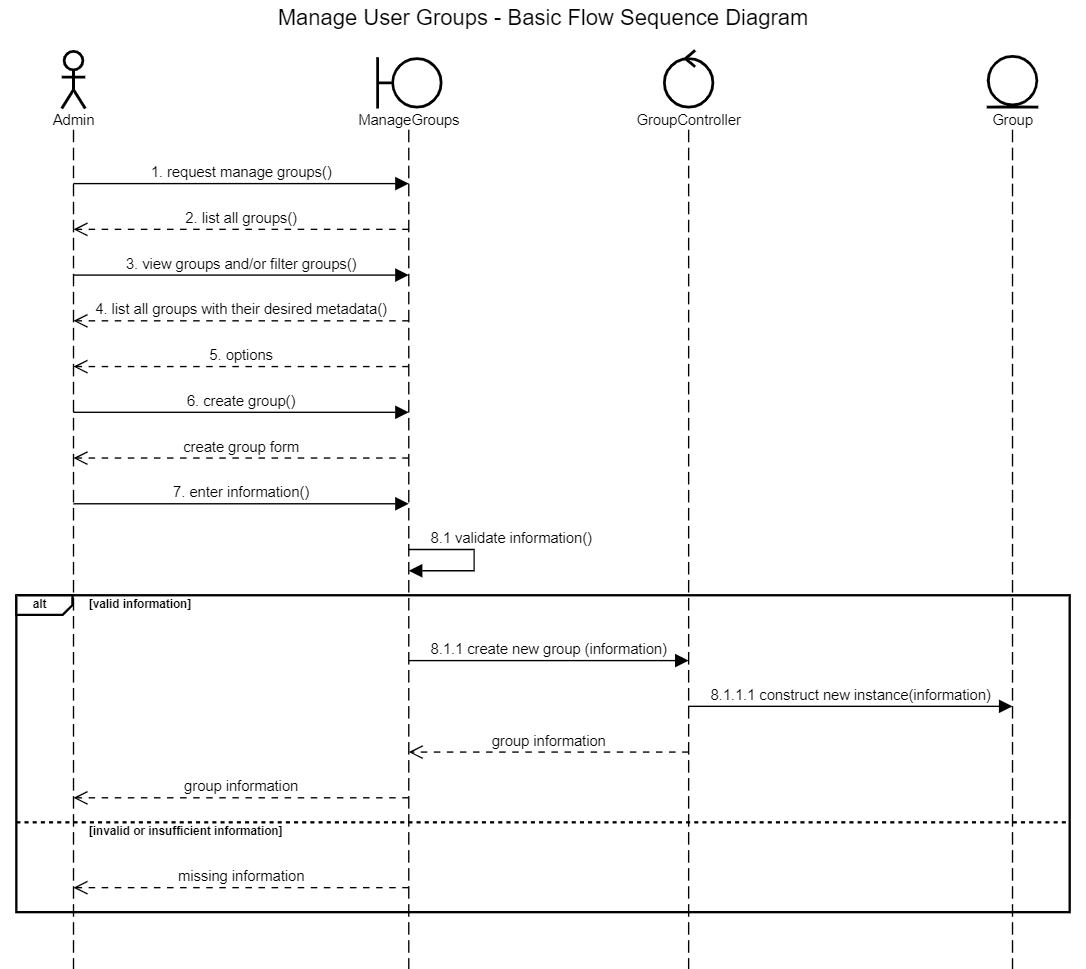
\includegraphics[width=1.0\textwidth]{images/Manage User Groups - Basic Flow Sequence Diagram.png}
    \caption{Manage Groups - Basic Flow Sequence diagram}
    \label{fig:SeqGroupsBasic}
\end{figure}
\subsubsection{Update Group - Sub flow}
If the Admin wishes to edit by selecting the target group, the system will display an update group[ form (Figure \ref{fig:adminUpdateGroup} in Appendices). After the Admin enters the updated information, the system will check if the group exists or not. If the group exists, the system will save the updated information of the group. If not, the system displays an error message. 
\begin{figure}[H]
    \centering
    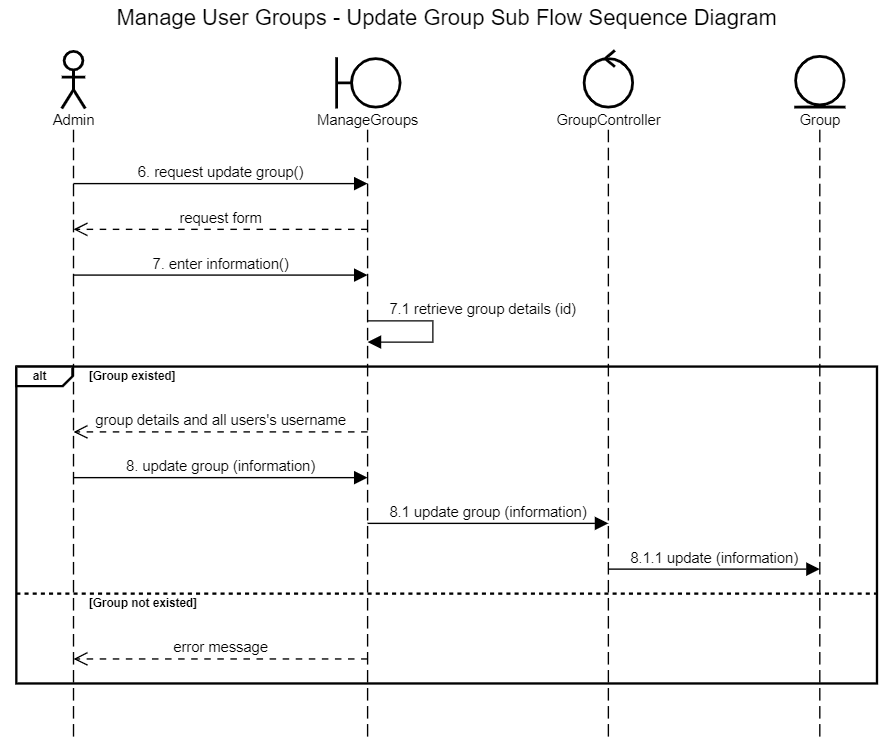
\includegraphics[width=1.0\textwidth]{images/Manage User Groups - Update Group Sub Flow Sequence Diagram.png}
    \caption{Manage User Groups - Update Group Sub Flow Sequence diagram}
    \label{fig:SeqGroupsUpdate}
\end{figure}
\subsubsection{Delete Group - Sub flow}
If the Admin wished to delete a group by selecting the target group, the system would display the full details of the group. When Admin clicks on the "Delete" button, the system will checks if the group exists or not. If the group exists, the system will remove the group. If not, the system displays an error message.
\begin{figure}[H]
    \centering
    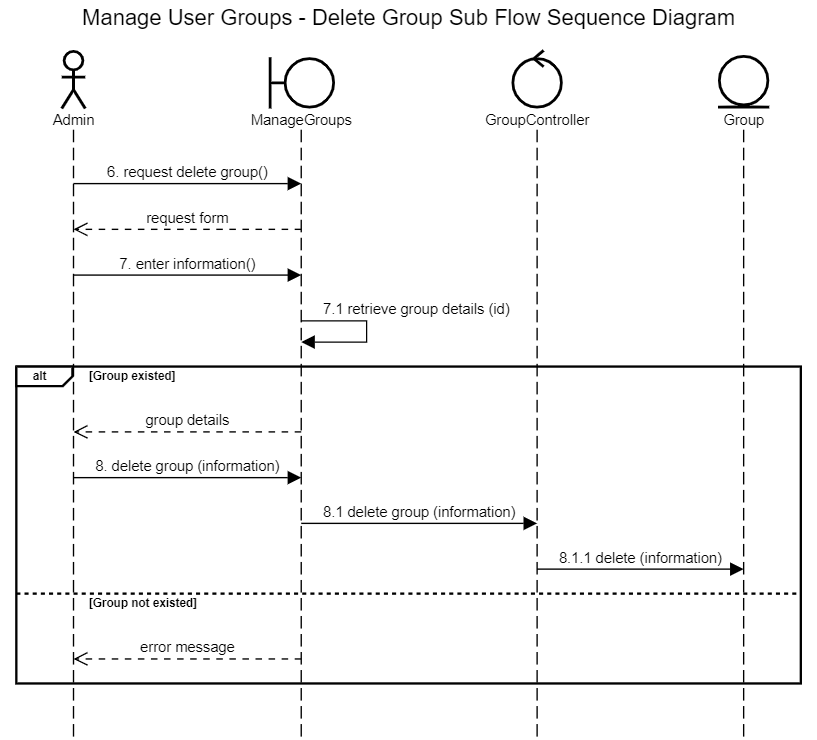
\includegraphics[width=1.0\textwidth]{images/Manage User Groups - Delete Group Sub Flow Sequence Diagram.png}
    \caption{Manage User Groups - Delete Group Sub Flow Sequence diagram}
    \label{fig:SeqGroupsDelete}
\end{figure}

\subsection{Manage Folders}
This Use Case describes how a User can manage folders.

\subsubsection{Manage Folders - Basic flow}
When the User logged into the system, the system lists all of the files and folders (Figure \ref{fig:listContent} in Appendices). The User can filter folders with desired criteria, and the system will respond to a list of folders. The User could choose to perform an action (create, edit, delete, move). If the User does not have permission to view a folder, that folder will not appear in the folder list. If the User chooses to create a folder, there will be a create folder form (Figure \ref{fig:createFolder} in Appendices). After the User enters all the required information, the system saves the folder information, assigns a unique id to the folder, and redirects to the files and folders interface. Otherwise, the system displays an error message and asks the User to re-enter the information. 

\begin{figure}[H]
    \centering
    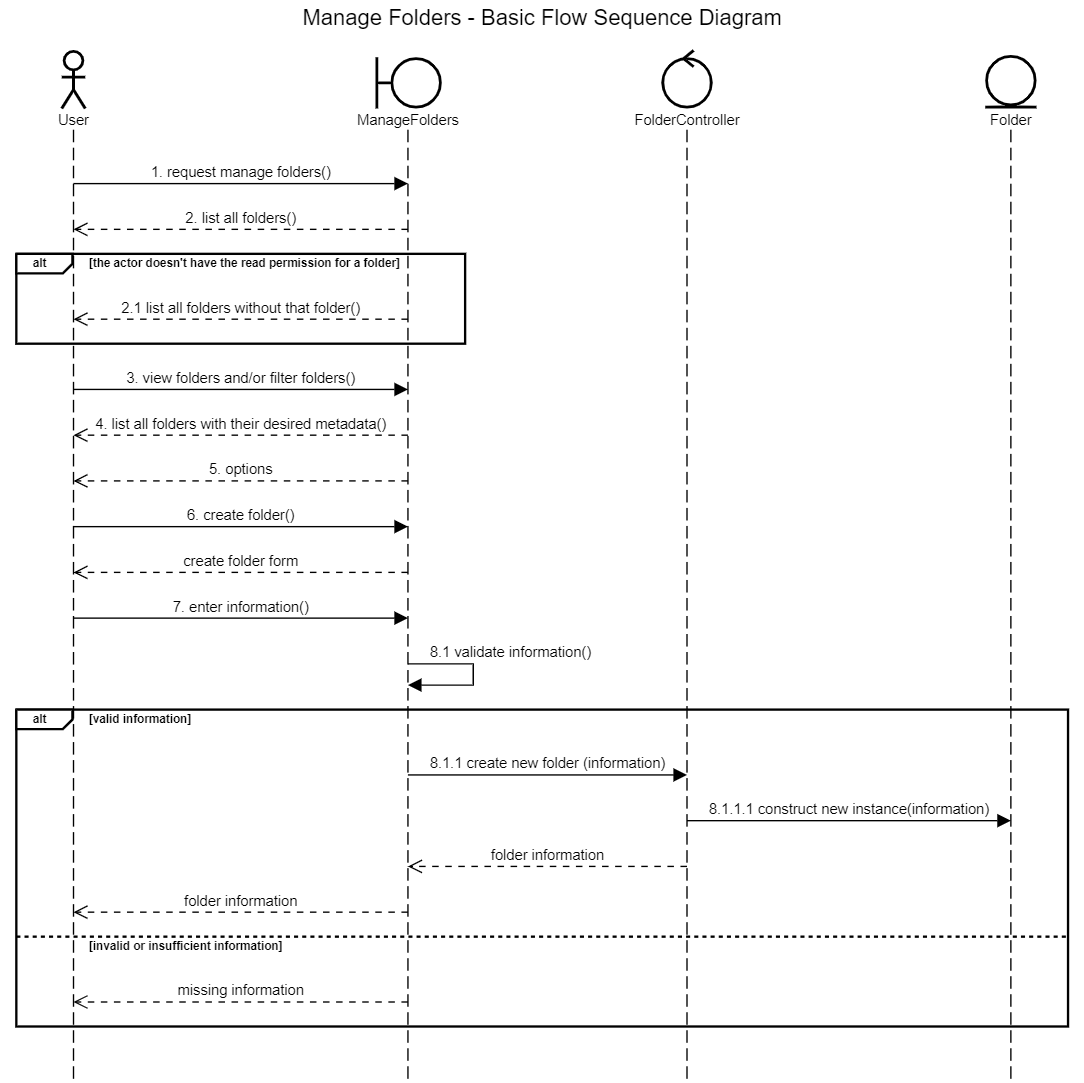
\includegraphics[width=1.0\textwidth]{images/Manage Folders - Basic Flow Sequence Diagram.png}
    \caption{Manage Folders - Basic Flow Sequence diagram}
    \label{fig:SeqFoldersBasic}
\end{figure}

\subsubsection{Update Folder - Sub flow}
If the User wishes to edit a folder by select the target folder, the system will check if the User have the right to write the folder. If the User does not have a write permission to a folder, the system will display en error message. Else, the system will display an update folder f\ref{fig:editFolder} in Appendices). After the User enters the updated information, the system will check if the folder exists or not. If the folder exists, the system will save the updated information of the folder. If not, the system displays an error message. 

\begin{figure}[H]
    \centering
    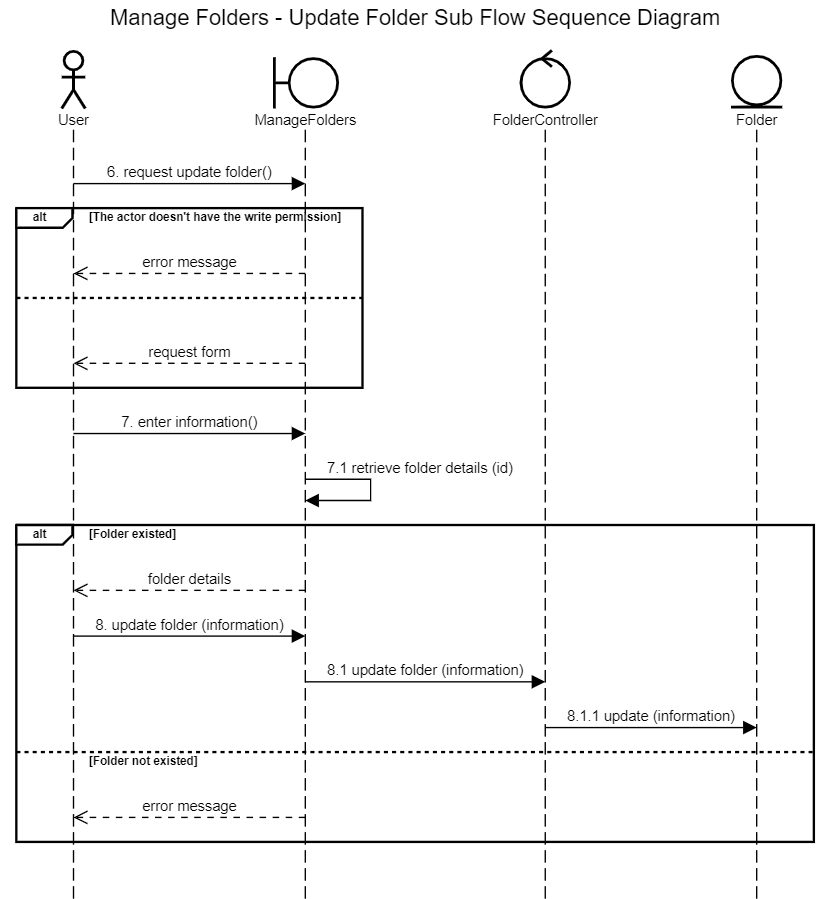
\includegraphics[width=1.0\textwidth]{images/Manage Folders - Update Folder Sub Flow Sequence Diagram.png}
    \caption{Manage Folders - Update Folder Sub Flow Sequence diagram}
    \label{fig:SeqFoldersUpdate}
\end{figure}

\subsubsection{Delete Folder - Sub flow}
If the User wished to delete a folder by selecting the target folder, the system will check if the User have the right to write the folder. If the User does not have a write permission to a folder, the system will display en error message. Else, the system would display the full details of the folder. When User clicks on the "Delete" button, the system will checks if the folder exists or not. If the folder exists, the system will remove the folder. If not, the system displays an error message.
\begin{figure}[H]
    \centering
    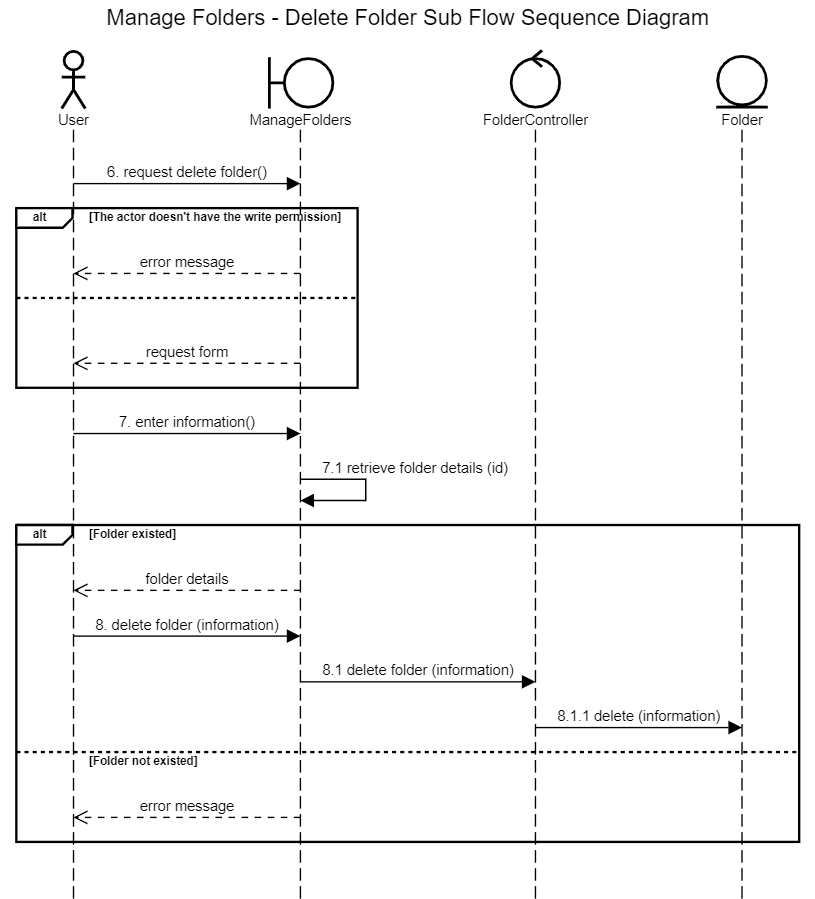
\includegraphics[width=1.0\textwidth]{images/Manage Folders - Delete Folder Sub Flow Sequence Diagram.png}
    \caption{Manage Folders - Delete Folder Sub Flow Sequence diagram}
    \label{fig:SeqFoldersDelete}
\end{figure}
\subsubsection{Move a Sub-folder a Folder - Sub flow}
If the User wishes to move a folder, the system will check if the User have the right to write the folder. If the User does not have a write permission to a folder, the system will display en error message. Else, the system will display a move folder form (Figure \ref{fig:moveContent}). The User will select a folder as source and enter the targeted folder and the destination folder. The system will move the targeted folder accordingly.  
\begin{figure}[H]
    \centering
    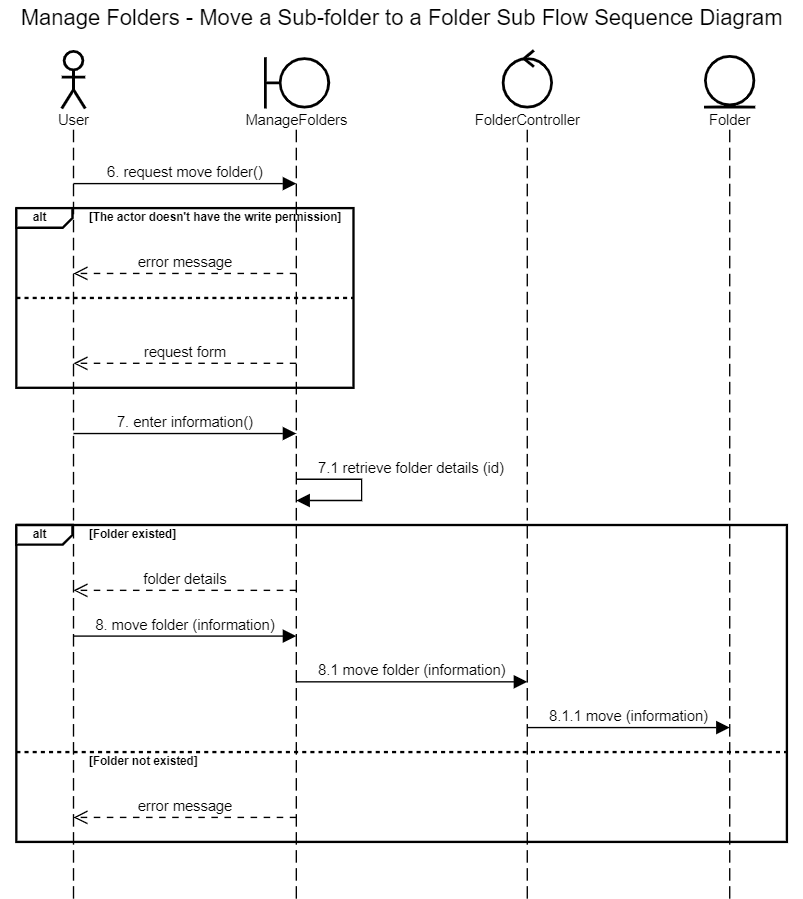
\includegraphics[width=1.0\textwidth]{images/Manage Folders - Move a Sub-folder to a Folder Sub Flow Sequence Diagram.png}
    \caption{Manage Folders - Move a Sub-folder to a Folder Sub Flow Sequence diagram}
    \label{fig:SeqFoldersMove}
\end{figure}

\subsection{Manage Files}
This Use Case describes how a User can manage files.
\subsubsection{Manage Files - Basic flow}
When the User logged into the system, the system lists all of the files and folders (Figure \ref{fig:listContent} in Appendices). The User can filter files with desired criteria, and the system will respond to a list of files. If the User does not have permission to view a file, that file will not appear in the file list. The User could choose to perform an action (upload, edit, delete, move, download). If the User chooses to upload, there will be an upload file form (Figure \ref{fig:uploadFile} in Appendices). After the User enters all the required information, the system saves the file information, assigns a unique id to the file, and redirects to the files and folders interface. Otherwise, the system displays an error message and asks the User to re-enter the information. 
\begin{figure}[H]
    \centering
    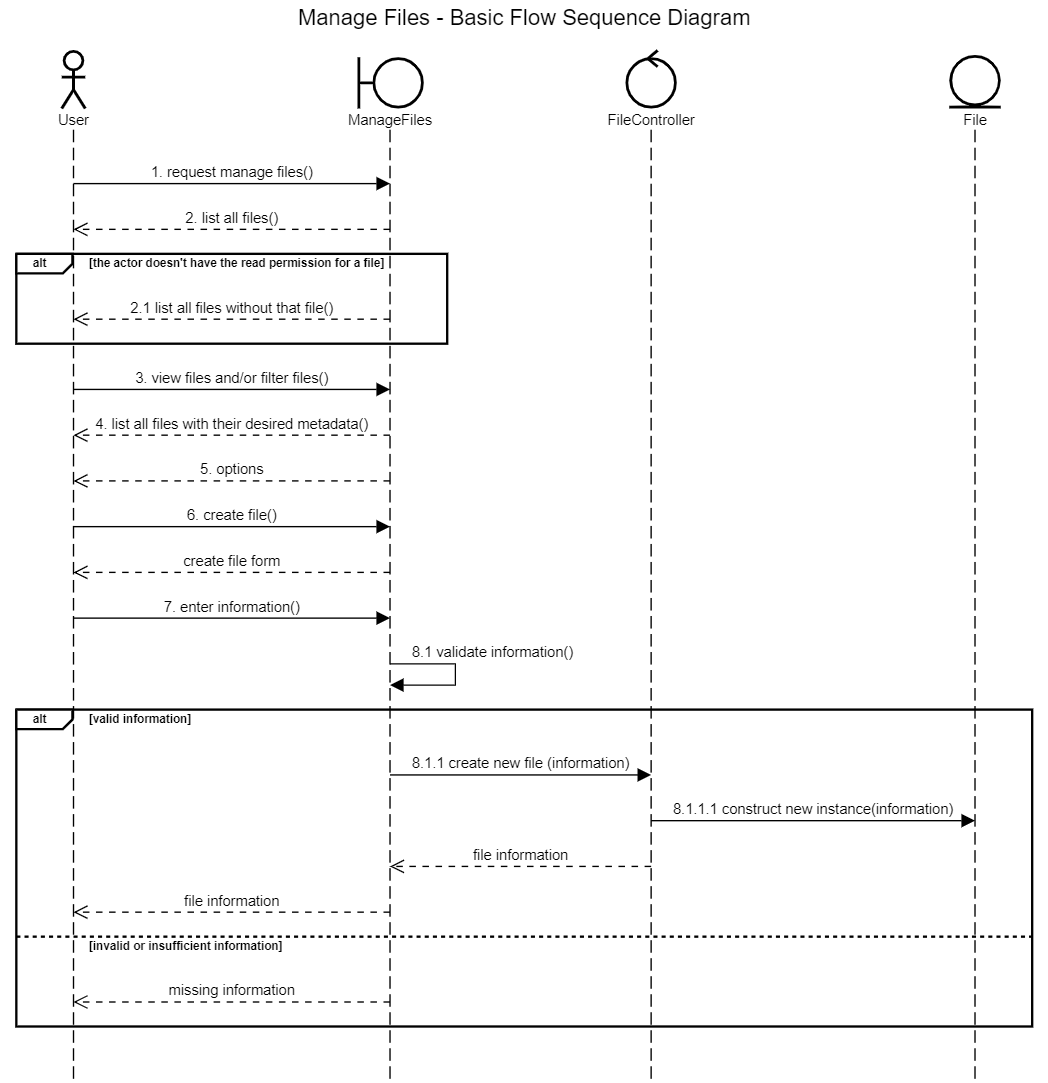
\includegraphics[width=1.0\textwidth]{images/Manage Files - Basic Flow Sequence Diagram.png}
    \caption{Manage Files - Basic Flow Sequence diagram}
    \label{fig:SeqFilesBasic}
\end{figure}
\subsubsection{Update File - Sub flow}
If the User wishes to edit a file by select the target file, the system will check if the User have the right to write the file. If the User does not have a write permission to a file, the system will displays en error message. Else, the system will display an update file f\ref{fig:editFile} in Appendices). After the User enters the updated information, the system will check if the file exists or not. If the file exists, the system will save the updated information of the file. If not, the system displays an error message. 

\begin{figure}[H]
    \centering
    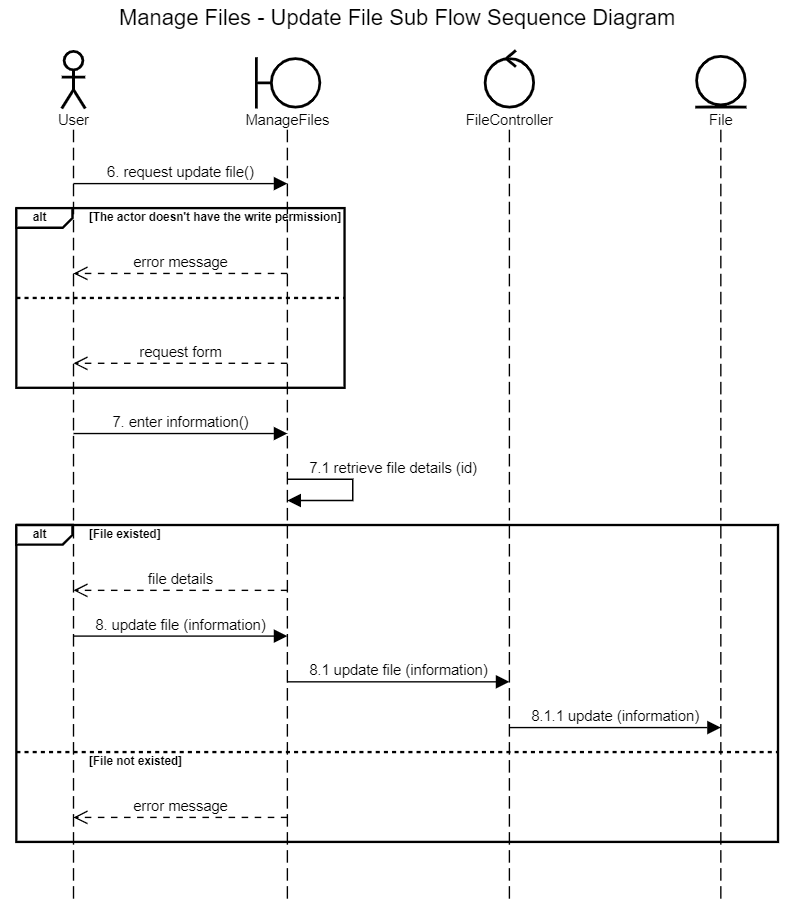
\includegraphics[width=1.0\textwidth]{images/Manage Files - Update File Sub Flow Sequence Diagram.png}
    \caption{Manage Files - Update File Sub Flow Sequence diagram}
    \label{fig:SeqFilesUpdate}
\end{figure}
\subsubsection{Delete File - Sub flow}
If the User wished to delete a file by selecting the target file, the system will check if the User have the right to write the file. If the User does not have a write permission to a file, the system would display an error message. Else, the system would display the full details of the file. When User clicks on the "Delete" button, the system will checks if the file exists or not. If the file exists, the system will remove the file. If not, the system displays an error message.
\begin{figure}[H]
    \centering
    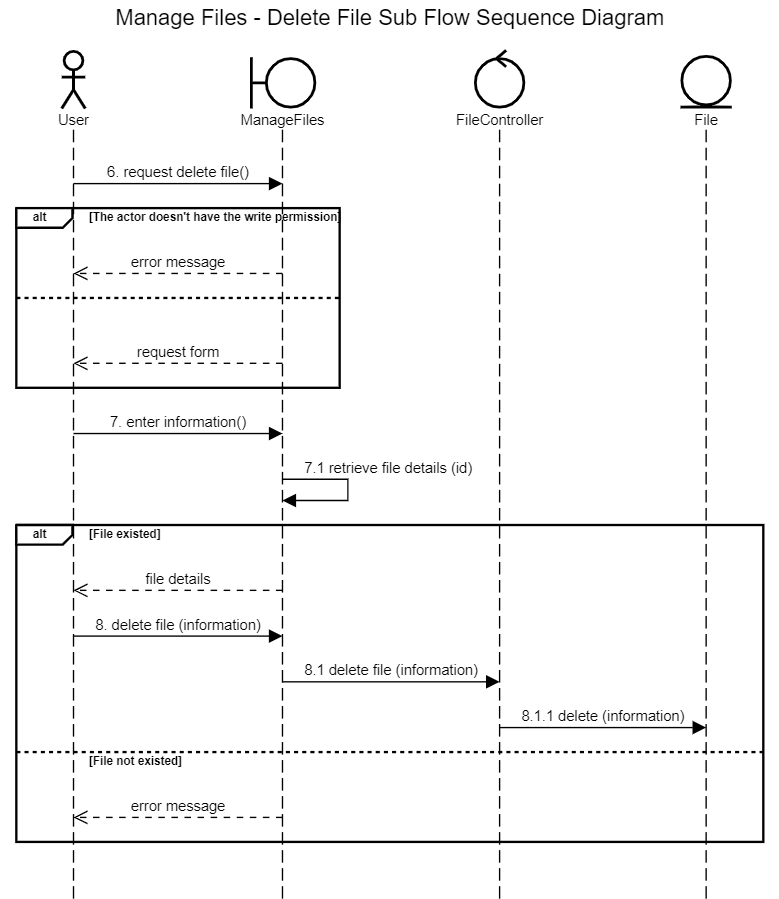
\includegraphics[width=1.0\textwidth]{images/Manage Files - Delete File Sub Flow Sequence Diagram.png}
    \caption{Manage Files - Delete File Sub Flow Sequence diagram}
    \label{fig:SeqFilesDelete}
\end{figure}
\subsubsection{Move a File a Folder - Sub flow}
If the User wishes to move a file, the system will check if the User have the right to write the file. If the User does not have a write permission to a file, the system will display an error message. Else, the system will display a move file form (Figure \ref{fig:moveContent}). The User will select a file as source and enter the targeted folder and the destination folder. The system will move the targeted file accordingly.  
\begin{figure}[H]
    \centering
    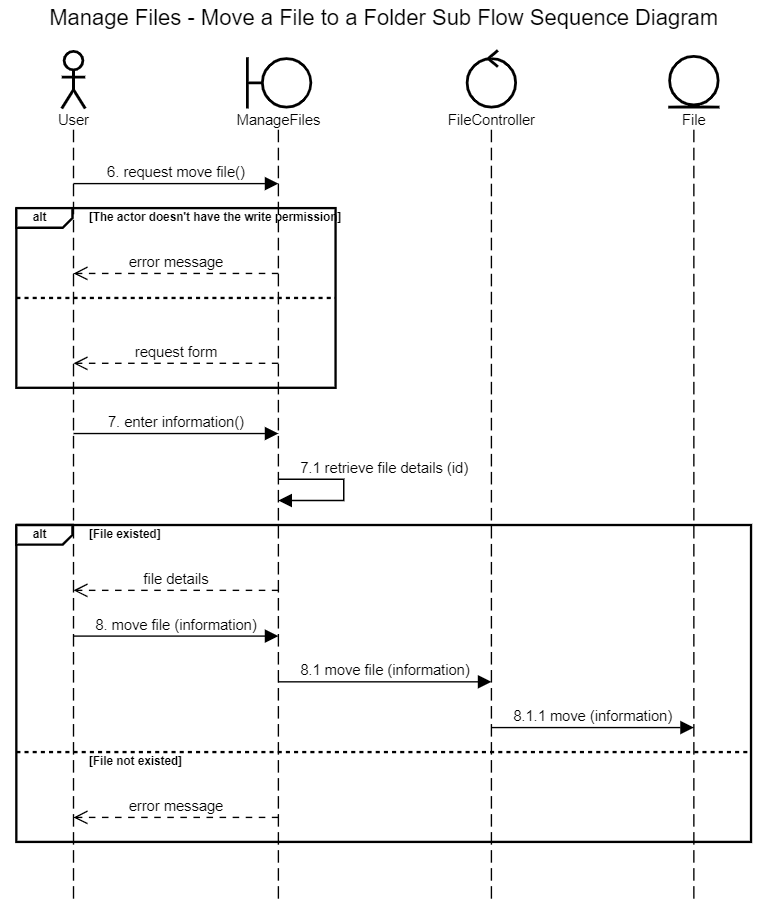
\includegraphics[width=1.0\textwidth]{images/Manage Files - Move a File to a Folder Sub Flow Sequence Diagram.png}
    \caption{Manage Files - Move a File to a Folder Sub Flow Sequence diagram}
    \label{fig:SeqFilesMove}
\end{figure}
\subsubsection{Download File - Sub flow}
If the User wishes to download a file, the system will check if the User have the right to view the file. If the User does not have a view permission to a file, the system will display an error message. Else, the system will process to return the file data for the user.  
\begin{figure}[H]
    \centering
    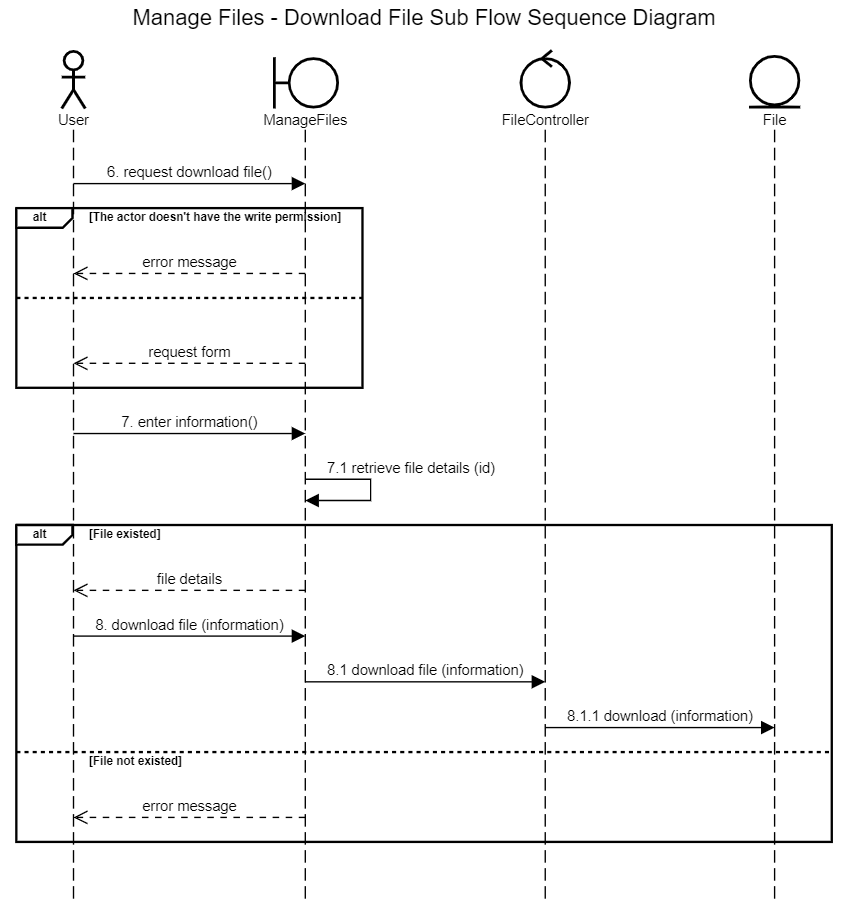
\includegraphics[width=1.0\textwidth]{images/Manage Files - Download File Sub Flow Sequence Diagram.png}
    \caption{Manage Files - Download File Sub Flow Sequence diagram}
    \label{fig:SeqFilesDownload}
\end{figure}

\subsection{Manage ACLs}
This Use Case describes how a User can manage ACLs permission.
\subsubsection{Manage ACLs - Basic flow}
In the selected file or folder, the User wishes to manage ACL permissions (grant or delete). If the User chooses to grant, there will be an grant ACL form (Figure \ref{fig:viewFile} and Figure \ref{fig:viewFolder} in Appendices). After the User enters all the required information, the system saves the ACL information, assigns a unique id to the ACL. Otherwise, the system displays an error message and asks the User to re-enter the information. 
\begin{figure}[H]
    \centering
    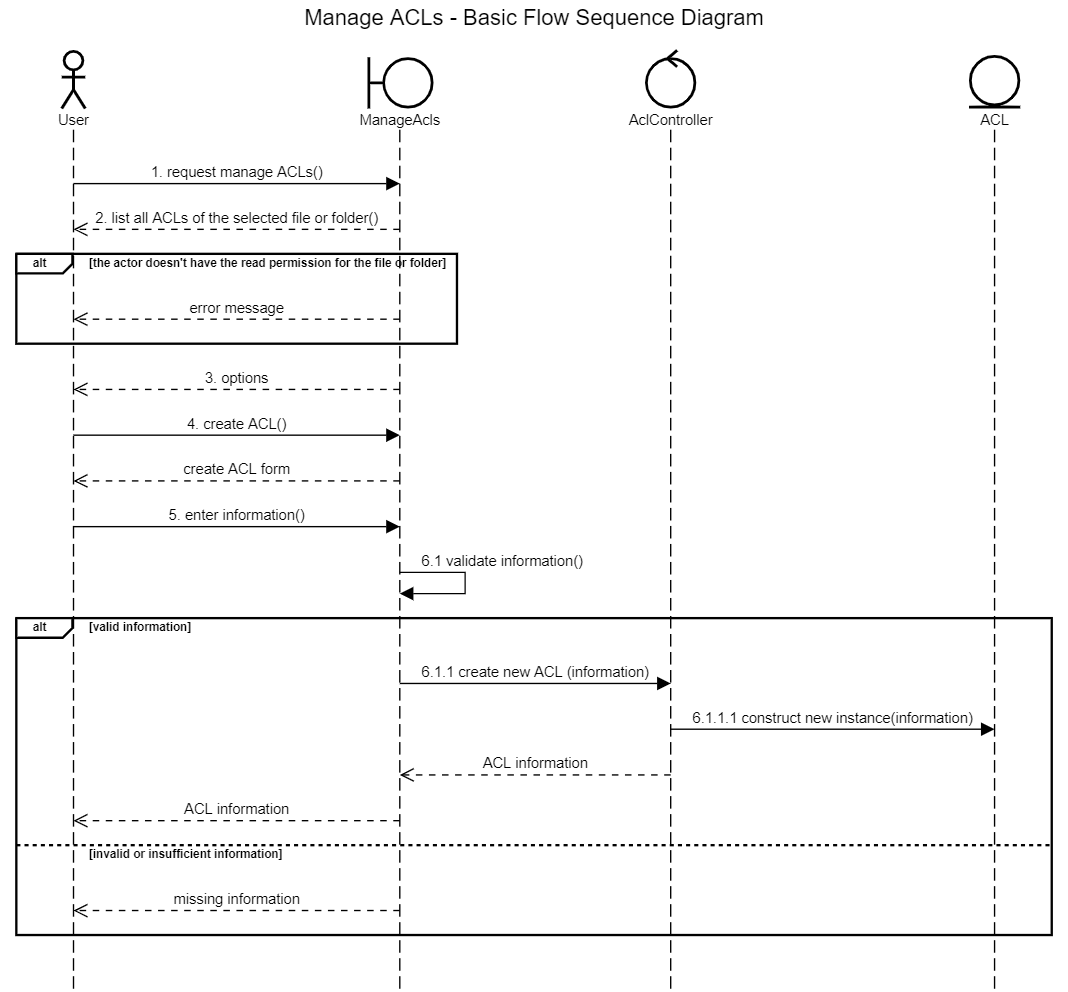
\includegraphics[width=1.0\textwidth]{images/Manage ACLs - Basic Flow Sequence Diagram.png}
    \caption{Manage ACLs - Basic Flow Sequence diagram}
    \label{fig:SeqACLsBasic}
\end{figure}
\subsubsection{Delete ACL - Sub flow}
If the User wished to delete a ACL by selecting the target ACL, the system will check if the User have the right to write the file or folder. If the User does not have a write permission, the system would display an error message. Else, the system would display the full details of the file or folder. When User clicks on the "Delete" button, the system will checks if the ACL exists or not. If the ACL exists, the system will remove the ACL. If not, the system displays an error message.
\begin{figure}[H]
    \centering
    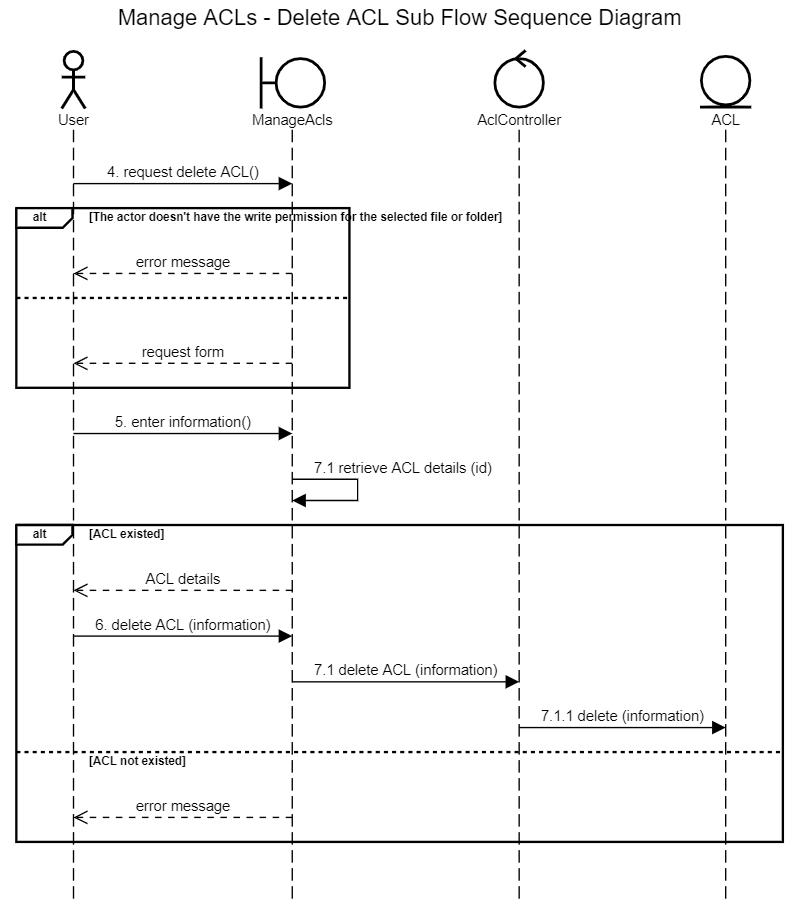
\includegraphics[width=1.0\textwidth]{images/Manage ACLs - Delete ACL Sub Flow Sequence Diagram.png}
    \caption{Manage ACLs - Delete ACL Sub Flow Sequence diagram}
    \label{fig:SeqACLsDelete}
\end{figure}

\section{Tools and Techniques}
\subsection{SQL}
With so much data and business relationships in our system, selecting a suitable database to manage it is critical. SQL is the clear choice because the project needs a close consistency between the data with high transactions and data security. While NoSQL has unstable schemas and is not fit for complex queries. Therefore, the best solution for our system is using SQL Database.\cite{mysql}

\subsection{Spring Boot}
Spring Boot is based on the Spring framework and has several dependencies that can be integrated into a Spring application. Spring Kafka, Spring LDAP, Spring Web Services, and Spring Security are some examples. \cite{spring}

Spring Boot uses Java, which is one of the most popular programming languages in the world. It reduces development time, increases the development team's overall productivity, and helps autoconfigure all components for a production-grade Spring application.

The dependency injection element of the Spring framework focuses on offering flexibility. It facilitates the injection of required dependencies and the development of a loosely linked application. It is a lightweight framework that is compatible with many middleware services.

\subsection{ReactJS}
React.js is an open-source JavaScript package to create single-page apps' user interfaces. For web and mobile apps, it is used to manage the view layer. We can also make reusable UI components with React. \cite{reactjs}
 
React allows developers to create large web applications that can change data without reloading the page. The primary purpose of React is to be fast, scalable, and straightforward. It works only on user interfaces in the application. This corresponds to the view in the MVC template. It can be used with other JavaScript libraries or frameworks, such as Angular JS in MVC.

There are so many open-source platforms for making front-end web application development more accessible, like Angular. React has some benefits over other competitive technologies or frameworks. The component-based approach, well-defined lifecycle, and plain JavaScript make React very simple to learn, build a professional web (and mobile applications), and support it. React uses a special syntax called JSX, which allows us to mix HTML with JavaScript. It has a better learning curve than Angular because Angular is a 'Domain-specific Language'. React only requires basic knowledge of CSS and HTML.

For this project, according to the condition and the requirement of the system environment, React is a great choice compared to others. 

\subsection{Axios}
Axios is a popular, promise-based HTTP client \cite{axios} that sports an easy-to-use API and can be used in both the browser and Node.js.

One of the most common activities a client-side JavaScript application will have to perform is making HTTP requests to fetch or save data. Third-party libraries have long been a popular approach to deal with more verbose browser APIs while abstracting away any variations across browsers.

Axios can be used in both the browser and Node.js compared with Fetch API built in many modern browsers. One such difference is in how the two libraries treat HTTP error codes \cite{http}. When using Fetch, if the server returns a 4xx or 5xx series error, the catch() callback will not be triggered, and it is down to the developer to check the response status code to determine if the request was successful. On the other hand, Axios will reject the request promise if one of these status codes is returned.

One distinction that may prove to be a deal-breaker for some is status updates on uploads and downloads. We may register callback functions for onUploadProgress and onDownloadProgress to display the percentage completion in the app's UI because Axios is built on top of the older XHR API. Fetch cannot currently do so. Therefore, the best choice is using Axios.

\subsection{Material-UI}
Material-UI is based on Google's Material Design guidelines. Like other design systems, Material Design was intended to provide a uniform user experience across various devices, platforms, and input methods. Google adopted Material Design to ensure that users had a uniform user experience regardless of how they accessed their products. Apple embraced flat design principles as their standard. \cite{material}

Material-UI is the world's most popular React UI framework. It provides a strong foundation for building dynamic UIs. It is blazing fast. It uses JSS at its core – a high performance JavaScript to CSS compiler which works at runtime and server-side, with less than 15 KB gzipped; and no bundle size increase if used alongside Material-UI.

\subsection{Swagger}
API Documentation is needed because the application is connected to many other services. It will improve user adaption, save support time and costs, and easier maintenance.

Swagger with API description formats like the OpenAPI/Swagger Specification is an excellent choice for that purpose. It has automated the documentation process, making it easier for teams to generate and maintain them. \cite{swagger}

\subsection{JWT (JSON Web Token)}
JWT is now widely used for authentication and data exchange. The Server encodes data into a JSON Web Token and transmits it to the Client instead of starting a Session (Session-based Authentication). After the Client saves the JWT, it should be appended to every request from the Client to protected routes or resources (commonly at header). The Server will validate the JWT, and the response will be returned.

Compared to Session-based Authentication, which requires the storage of the session on a cookie, JWT (Token-based Authentication) has the substantial advantage of storing the token on the client-side: Local Storage for browsers, Keychain for iOS, and SharedPreferences for Android... As a result, we will not need to create a separate backend project for Native Apps or a separate Authentication module for Native App users. 

For that, using JWT is ideal for this project.

\subsection{RBAC and ACL Authorization}
We developed the authentication from JWT, which establishes the principal's identity. After then, authorization is required, which determines what the principal is permitted to do. We start with role-based authorization (RBAC), which involves assigning roles to specific users and then utilizing those roles to define what they may see and do, ideally through related permissions. Role Admin and Role User are two types of roles. 

When we have to maintain predicates on principals regarding specific targets, the problem occurs. When we discuss the data lake, we want to make it so that only the file owner and the admin may update a file after it has been posted and that no one else can do so without authorization. "Can User1 edit files in general?" is a question that role-based permission helps us answer. ACL-based authorization (Access Control List) is more fine-grained, requiring the management of relationships between actors and targets to answer the question, "Can User1 edit file 10?". \cite{authorization}

We implement ACL Authorization Model with the help of Spring Security's ACL module. 